\section{FUNDAMENTOS DE LOS SISTEMAS DE RECOMENDACIÓN: }

Los sistemas de recomendación son \textbf{agentes de información personalizada} que brindan sugerencias de elementos que \textit{podrían} ser útiles para un usuario.  Los resultados dados por un sistema de recomendación se denominan \textbf{Recomendaciones} que representan una opción valiosa que podría ser del interés de una persona o usuario.

\subsection{CONCEPTOS BÁSICOS DE LOS SISTEMAS DE RECOMENDACIÓN: }

Los Sistemas de Recomendación se fundamentan mediante entidades que aportan información desde diferentes medios:

\begin{itemize}
    \item \textbf{Usuario: } La entidad a la que se le hacen llegar las recomendaciones es denominada como \textit{usuario}. 
    \item \textbf{Items: } Es una pieza de información que refiere a un objeto tangible o digital que el sistema de recomendación sugerirá al usuario en una interacción a través de la Web, email o mensajes de texto \parencite{Kotkov2020Serendipity}.
    \item \textbf{Fuente de Conocimiento: } Determina qué técnica será usada para definir el medio de información y determinar el conocimiento necesario para brindar sugerencias relevantes.
\end{itemize}

El principio básico que fundamenta a los algoritmos de recomendación es la dependencia significativa que existe entre un \textit{usuario} y los \textit{items} con los que interactúa.

\newpage
\thispagestyle{plain}
\vspace*{0.2cm}

\subsection{OBJETIVOS DE UN SISTEMA DE RECOMENDACIÓN: }
Según \parencite{Aggarwal2016} más allá de los objetivos mercadológicos que se le atribuyen a los sistemas de recomendación enfocados en mejorar el rendimiento económico de una plataforma, se pueden definir objetivos técnicos y operacionales que mejoran el rendimiento de un sistema en éste ámbito.

\begin{itemize}
    \item \textbf{Relevancia: }Un sistema de recomendación siempre debe brindar sugerencias relevantes para el usuario.
    \item \textbf{Novedad: }  Las recomendaciones suelen ser más útiles cuando sugieren elementos que el usuario no ha visto antes. Además, recomendar los objetos más populares puede conducir a reducir la diversidad del consumo.
    \item \textbf{Sorpresa: } No basta con que los objetos de recomendación sean nuevos para el usuario, sino que también deben sorprenderlo, dándole la sensación de un \textit{descubrimiento inesperado.}
    
    \item \textbf{Diversidad de Recomendaciones: } La lista de sugerencias obtenidas deben ser suficientemente diferentes entre sí para no aburrir al usuario, sin embargo, la diversidad de \textit{items} no debe alejarse demasiado de sus preferencias.
   \enquote{\textit{La diversidad tiene el beneficio de asegurar que el usuario no se aburre de constantes recomendaciones de items similares. }} [\cite{Aggarwal2016}]
\end{itemize}

Existen dos versiones diferentes que definen los resultados esperados de un Sistema de Recomendación, ambos buscan resolver el problema de encontrar items relevantes para los usuarios mediante modelos distintos:


\begin{enumerate}
    \item \textbf{Versión de Predicción: } Se basa en predecir la calificación que el usuario daría a un item. Se asume que existe un conjunto de Datos de Entrenamiento que indica las preferencias del usuario.
    \item \textbf{Versión de Top - $k$: } Este enfoque argumenta que muchos de los sistemas no necesitan conocer la calificación estimada del usuario, por el contrario, solo necesitan saber qué recomendar sin necesidad de estimar una calificación exacta. Esto se suele hacer mediante un Top - $k$ elementos que probablemente le gusten al usuario.
\end{enumerate}

\newpage
\thispagestyle{plain}
\vspace*{0.2cm}

\subsection{PRINCIPALES ENFOQUES DE RECOMENDACIÓN: }
Para que un sistema de recomendación logre cumplir los objetivos básicos esperados se necesita establecer de forma clara cuál será el filtro para sugerir items al usuario eligiendo diferentes enfoques que se adapten a los resultados que se buscan obtener.

Basándose en \parencite{ISINKAYE2015261} existen diferentes filtros de recomendación principales, sin embargo, se muestran los más relevantes para el presente proyecto:

\subsubsection{ENFOQUE BASADO EN CONTENIDO: }
Es una técnica de sistema de recomendación que se centra en el análisis de atributos de cada item para generar predicciones sobre las preferencias del usuario. Se apoya de valoraciones previamente vinculadas a un perfil que permiten identificar características clave de los objetos que el usuario ha calificado, principalmente de aquellos que cuentan con una valoración positiva.  Por esta razón, la eficacia de este enfoque se basa en la cantidad de información disponible de los items.

Los algoritmos que implementan esta técnica suelen basarse en modelos de análisis estadístico y de \textit{Machine Learning.}

\textbf{VENTAJAS: }
\begin{itemize}

    \item \textbf{Capacidad recomendar items nuevos: } Este enfoque permite sugerir elementos que aún no han sido evaluados por los usuarios gracias a la información contenida en sus \textit{metadatos} \footnote{\textbf{Metadatos: } Atributos que describen, proveen contexto, indican la calidad, o documentan las características de un objeto. \parencite{Greenberg09092005}}.
    \item \textbf{Alta adaptabilidad: } Se adapta a los cambios de preferencia del usuario en un lapso corto de tiempo.

    \item \textbf{Independencia entre usuarios: } Los usuarios reciben recomendaciones sin la necesidad de compartir su información con externos, priorizando la privacidad y seguridad de los datos.
    
\end{itemize}

\newpage
\thispagestyle{plain}
\vspace*{0.2cm}

\textbf{DESVENTAJAS: }
\begin{itemize}

    \item \textbf{Dependencia en la profundidad de la información: } Los motores de recomendación basados en esta técnica son dependientes de los metadatos vinculados a los items. Por lo tanto, requieren que los elementos sean profundamente descritos por sus atributos. Esto es definido como \textbf{\textit{Análisis limitado al contenido}}.
    
    \item \textbf{Falta de Diversidad: } Es probable que las sugerencias sufran de \textit{sobre-especialización} o, en otras palabras, que carezcan de diversidad debido a que los usuarios están restringidos a obtener recomendaciones similares a los items asociados a sus perfiles.
\end{itemize}

\newpage
\thispagestyle{plain}
\vspace*{0.2cm}

\textbf{ENFOQUE COLABORATIVO:}

A diferencia del enfoque basado en contenido, que se centra en los atributos de los items, el enfoque colaborativo se centra en las similitudes entre lo usuarios para generar recomendaciones.

Este enfoque funciona construyendo una base de datos descrita por una matríz \textit{usuarios - items} que representa la preferencia de un conjunto de usuarios por un item particular. Este enfoque vincula a diferentes perfiles con preferencias e intereses similares para guiar las recomendaciones, formando así un grupo  de perfiles que comparten intereses denominado \textit{Vecindario}. 


Por lo tanto, un usuario recibe recomendaciones de contenido que no ha evaluado pero que otros usuarios dentro de su \textit{Vecindario} han calificado de forma positiva. Los resultados que se pueden obtener a través de este enfoque son los siguientes:

\begin{itemize}
    \item \textbf{Predicciones: } Es un valor numérico que expresa un puntaje del elemento $j$ para el usuario $i$, esta predicción se representa con la notación $R_{i,j}$.
    \item \textbf{Recomendaciones: } Es una lista de los Top - $N$ elementos que al usuario le podrían gustar más.
\end{itemize}

\begin{figure}[h!]
    \centering
    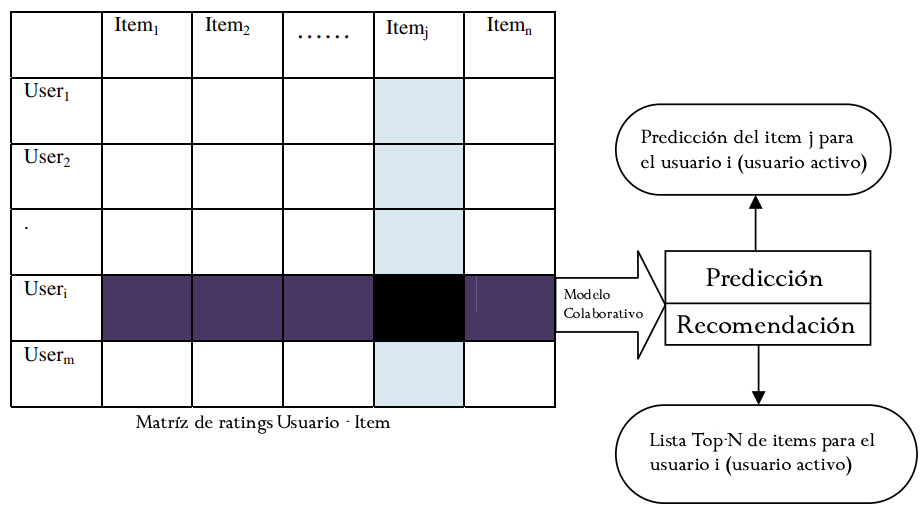
\includegraphics[width=0.7\linewidth]{FiltroBasadoenContenido.png}
    \caption{Ejemplo del Filtro Basado en Colaboración \parencite{ISINKAYE2015261}.}
    \label{fig:FiltroColaborativo}
\end{figure}

\newpage
\thispagestyle{plain}
\vspace*{0.2cm}


En la figura \ref{fig:FiltroColaborativo} se muestra un ejemplo de funcionamiento del enfoque colaborativo. Se puede observar que la matríz está compuesta por filas que representan a los usuarios de un mismo \textit{Vecindario}, y por columnas que representan a los \textit{items}. Las intersecciones mostradas de color morado representan la calificación que el usuario ha dado a elementos previos, y la intersección diferenciada de color negro expresa una predicción basada en las calificaciones que los vecinos han asignado a ese item.
El diagrama remarca la distinción entre \textit{Predicción} y la \textit{Recomendación} dado que, en el caso de la predicción,  la intersección representada en color negro representa el valor $R_{i,j}$, y en el caso de la recomendación representa un \textit{item} dentro de los Top - $N$ items del usuario actual.

\textbf{VENTAJAS:}


Este enfoque tiene ventajas fuertemente diferenciadas respecto al enfoque basado en contenido, algunos de sus puntos fuertes son los siguientes:

\begin{itemize}
    \item \textbf{Independencia al Contenido: } Este enfoque puede funcionar de forma efectiva en dominios en los cuales no existe diversidad de información (o metadatos) para describir los items.
    \item \textbf{Recomendaciones basadas en Serendipia \footnote{\textbf{Serendipia en Sistemas de Recomendación: } \textit{Items} que son relevantes pero inesperados para el usuario. \textit{Items} que son nuevos e inesperados. \parencite{Kotkov2020Serendipity}} }: Este enfoque tiene la capacidad de recomendar elementos que son aparentemente ajenos a las preferencias del usuario, pero que para sus \textit{vecinos} son relevantes, conectando al usuario con contenido nuevo.
\end{itemize}

\textbf{DESVENTAJAS:}

\begin{itemize}
    \item \textbf{Problema de \textit{Inicio Frío}}: Se refiere a la situación en donde el Sistema de Recomendación no tiene información adecuada acerca del usuario o acerca del item para hacer predicciones relevantes \parencite{Burke2007}. Este problema es crucial ya que este enfoque se vuelve dependiente de conocer con el tiempo las preferencias del usuario que, inicialmente, son desconocidas.

    \item \textbf{Problema del \textit{Esparcimiento de Datos}}: Otro de los puntos de los que depende el enfoque colaborativo es en las calificaciones hechas por los usuarios, causando la necesidad de que existan previas valoraciones para los items, de lo contrario, se generan recomendaciones poco relevantes.
\end{itemize}

\newpage
\thispagestyle{plain}
\vspace*{0.2cm}
\begin{itemize}
    \item \textbf{Escalabilidad}: Un problema bastante común en los algoritmos de recomendación con enfoque colaborativo es la escalabilidad. Cuando la cantidad de usuarios e items crecen rápidamente, la complejidad computacional crece de forma lineal en relacion a estos dos aspectos, dando un costo computacional representado por la siguiente fórmula: $O(items \ \cdot \ usuarios)$\footnote{\textbf{Notación \textit{BIG O}:}  Es un estándar que describe el orden de crecimiento de un algoritmo en función del tamaño del problema. En el presente documento se usará para expresar la complejidad computacional de los algoritmos descritos.}. Es importante mencionar que un algoritmo lineal no logra ser eficaz cuando la cantidad de información es masiva.

    \item \textbf{\textit{Sinónimos: }} Se refiere a la situación en la que items muy similares aparecen registrados con diferentes nombres o identificadores \parencite{ISINKAYE2015261}. Los sistemas de colaboración no reconocen automáticamente que se trata de equivalencias; por ejemplo, \textit{item 1: Álbum Let It Be - The Beatles}, \textit{item 2: Álbum Let It Be (Remasterizado) - The Beatles}. En este caso, el sistema podría tratarlos como elementos completamente diferentes, a pesar de estar estrechamente relacionados.
\end{itemize}

\newpage
\thispagestyle{plain}
\vspace*{0.2cm}

\textbf{ENFOQUE HÍBRIDO: }

A pesar de que los enfoques de recomendación basados en contenido y colaborativos son eficaces en escenarios particulares, sus desventajas inherentes limitan su escalabilidad en plataformas de uso masivo.  El enfoque híbrido busca solventar las desventajas de cada enfoque combinando diferentes técnicas de recomendación con el objetivo de evitar las limitaciones y problemas que los enfoques puros pueden enfrentar.

Los sistemas de recomendación híbridos están fuertemente relacionados al campo del \textit{Análisis de Conjuntos (Ensemble Analysis)} en los cuales se combina el poder de multiples tipos de algoritmos basados en \textit{Machine Learning} para crear modelos más robustos \parencite{Aggarwal2016}.  

\textbf{TÍPOS DE ENFOQUES HÍBRIDOS: }
\begin{itemize}
    \item \textbf{Enfoque Híbrido basado en Pesos: } Este enfoque combina los resultados de diferentes enfoques de recomendación para crear una lista de recomendaciones que integran las calificaciones de cada técnica mediante una fórmula lineal. Inicialmente todas las técnicas usadas inician con un peso igualado que se modifica a través de la evaluación del usuario.
    \item \textbf{Enfoque Híbrido por Conmutación: } Este enfoque se basa en una heurística definida que selecciona la mejor técnica de recomendación adaptada al momento. Por ejemplo, si se necesita de un algoritmo de recomendación para un usuario nuevo, se puede identificar que usar el enfoque colaborativo no es una buena opción debido al \textit{Inicio Frío}, por lo tanto, se elige el enfoque basado en contenido. El beneficio de esta estrategia es que el sistema es sensible a las fortalezas y debilidades de sus enfoques de recomendación \parencite{ISINKAYE2015261}. 

    Sin embargo, esta conmutación de enfoques tiene una desventaja inherente debido al costo computacional que requiere el cambiar de métodos constantemente, principalmente por la diferencia de criterios y parámetros de información que cada enfoque requiere.

    \item \textbf{Enfoque Híbrido Combinado: } Este enfoque combina los resultados de diferentes algoritmos de recomendación, ejecutándolos en paralelo para generar una lista única de recomendaciones. El beneficio principal de esta estrategia es que el rendimiento local de un enfoque específico no suele afectar de manera significativa al rendimiento global del sistema, resultando en una mayor robustez.
    
\end{itemize}